\documentclass[a4paper]{article}
\addtolength{\hoffset}{-2.25cm}
\addtolength{\textwidth}{4.5cm}
\addtolength{\voffset}{-3.25cm}
\addtolength{\textheight}{5cm}
\setlength{\parskip}{0pt}
\setlength{\parindent}{0in}

\usepackage[square,sort,comma,numbers]{natbib}
\usepackage{blindtext} % Package to generate dummy text
\usepackage{charter} % Use the Charter font
\usepackage[utf8]{inputenc} % Use UTF-8 encoding
\usepackage{microtype} % Slightly tweak font spacing for aesthetics
\usepackage{amsthm, amsmath, amssymb} % Mathematical typesetting
\usepackage{float} % Improved interface for floating objects
\usepackage{hyperref} % For hyperlinks in the PDF
\usepackage{graphicx, multicol} % Enhanced support for graphics
\usepackage{xcolor} % Driver-independent color extensions
\usepackage{pseudocode} % Environment for specifying algorithms in a natural way
\usepackage[mmddyy]{datetime} % Uses YEAR-MONTH-DAY format for dates

\usepackage{fancyhdr} % Headers and footers
\pagestyle{fancy} % All pages have headers and footers
\fancyhead{}\renewcommand{\headrulewidth}{0pt} % Blank out the default header
\fancyfoot[L]{} % Custom footer text
\fancyfoot[C]{} % Custom footer text
\fancyfoot[R]{\thepage} % Custom footer text
\newcommand{\note}[1]{\marginpar{\scriptsize \textcolor{red}{#1}}} % Enables comments in red on margin

\DeclareMathOperator*{\argmin}{arg\,min}

%----------------------------------------------------------------------------------------

\newcommand{\yourname}{Balthazar Neveu}
\newcommand{\youremail}{balthazarneveu@gmail.com}
\newcommand{\assignmentnumber}{4}

\begin{document}

\fancyhead[C]{}
\hrule \medskip
\begin{minipage}{0.295\textwidth} 
\raggedright
\footnotesize
\yourname \hfill\\
\youremail
\end{minipage}
\begin{minipage}{0.4\textwidth} 
\centering 
\large 
Lab session \# \assignmentnumber\\ 
\normalsize 
ALTEGRAD 2023\\ 
\end{minipage}
\begin{minipage}{0.295\textwidth} 
\raggedleft
\today\hfill\\
\end{minipage}
\medskip\hrule 
\bigskip


\section*{Code}
For part 1, I set up a 4 CPU TensorDock remote machine to avoid working on my local machine.
This took some time. Pre-requisite setup.sh \& download\_models.sh .

More info:
\href{https://github.com/balthazarneveu/MVA23_ALTEGRAD/#readme}{MVA ALTEGRAD Balthazar Neveu on Github}

\begin{itemize}
    \item code/fine\_tune\_roberta.ipynb : part 1 - trained on 4 CPU TensorDock remote machine.
    \item code/fine\_tune\_bloom.ipynb : part 2 - trained on Google Collab
\end{itemize}

\section{Fine tuning Roberta\cite{liu2019roberta}}
\subsection*{Question 1 \& Task 1: Model size}
I used the \textit{sympy} library to compute the number of parameters in the model analytically.
In the notebook we can compare that the number of parameters computed analytically is the same as the number of parameters computed using the \textit{torch.numel}..


When we check the RobertaSmall definition, we can read the following information, which follow the RoBerta\cite{liu2019roberta} paper convention.
\begin{verbatim}
ntokens = 32000 # -> V = vocabulary size
encoder_layers = nlayers = 4 # -> L = number of (attention+feedforward) transformer unit layers
encoder_embed_dim = 512 # -> D = embedding "feature" dimensions
encoder_ffn_embed_dim = 512 # -> D = feature dimensions used in the feed forward network
encoder_attention_heads = nhead = 8 # -> A = number of attentio heads
max_positions = 256 # -> T = max length of a sentence
\end{verbatim}


\begin{figure}[ht]
    \centering
    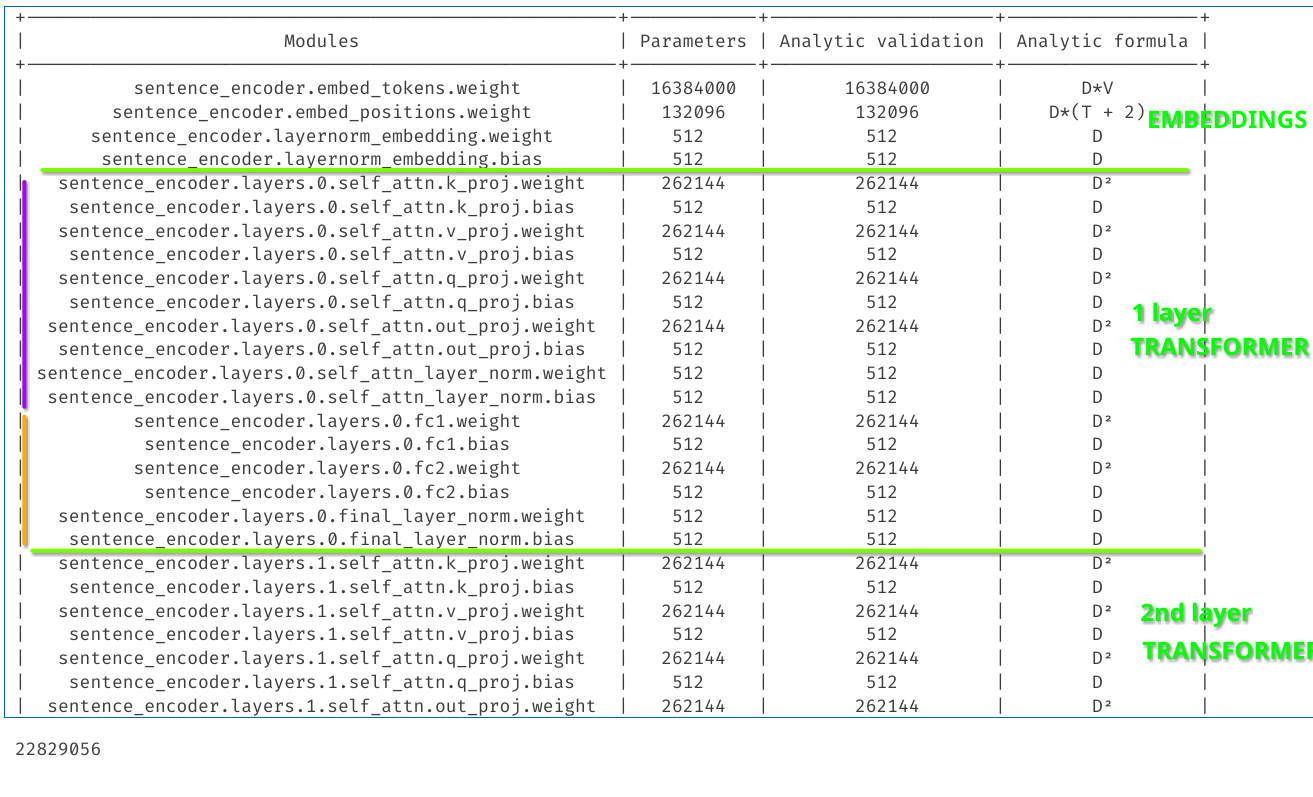
\includegraphics[width=.6\textwidth]{figures/roberta_params.png}
    \caption{Evaluating the number of parameters in the Roberta Small model, analytically and comparing to numerical values. \\ 
    Embedding layer is followed by $L=4$ Transformer units. Each Transformer unit is composed of a self-attention layer (in purple) and 2 feed forward layers (in orange)}
    \label{fig:roberta_params}
\end{figure}

\break 
\begin{tiny}
\begin{verbatim}

        +-------------------------------------------------------+------------+---------------------+------------------+
        |                        Modules                        | Parameters | Analytic validation | Analytic formula |
        +-------------------------------------------------------+------------+---------------------+------------------+
        |          sentence_encoder.embed_tokens.weight         |  16384000  |       16384000      |       D*V        |
        |        sentence_encoder.embed_positions.weight        |   132096   |        132096       |    D*(T + 2)     |
        |      sentence_encoder.layernorm_embedding.weight      |    512     |         512         |        D         |
        |       sentence_encoder.layernorm_embedding.bias       |    512     |         512         |        D         |
        +-------------------------------------------------------+------------+---------------------+------------------+
        |   sentence_encoder.layers.0.self_attn.k_proj.weight   |   262144   |        262144       |        D²        |
        |    sentence_encoder.layers.0.self_attn.k_proj.bias    |    512     |         512         |        D         |
        |   sentence_encoder.layers.0.self_attn.v_proj.weight   |   262144   |        262144       |        D²        |
        |    sentence_encoder.layers.0.self_attn.v_proj.bias    |    512     |         512         |        D         |
        |   sentence_encoder.layers.0.self_attn.q_proj.weight   |   262144   |        262144       |        D²        |
        |    sentence_encoder.layers.0.self_attn.q_proj.bias    |    512     |         512         |        D         |
        |  sentence_encoder.layers.0.self_attn.out_proj.weight  |   262144   |        262144       |        D²        |
        |   sentence_encoder.layers.0.self_attn.out_proj.bias   |    512     |         512         |        D         |
        | sentence_encoder.layers.0.self_attn_layer_norm.weight |    512     |         512         |        D         |
        |  sentence_encoder.layers.0.self_attn_layer_norm.bias  |    512     |         512         |        D         |
        |          sentence_encoder.layers.0.fc1.weight         |   262144   |        262144       |        D²        |
        |           sentence_encoder.layers.0.fc1.bias          |    512     |         512         |        D         |
        |          sentence_encoder.layers.0.fc2.weight         |   262144   |        262144       |        D²        |
        |           sentence_encoder.layers.0.fc2.bias          |    512     |         512         |        D         |
        |   sentence_encoder.layers.0.final_layer_norm.weight   |    512     |         512         |        D         |
        |    sentence_encoder.layers.0.final_layer_norm.bias    |    512     |         512         |        D         |
        +-------------------------------------------------------+------------+---------------------+------------------+
        |   sentence_encoder.layers.1.self_attn.k_proj.weight   |   262144   |        262144       |        D²        |
        |    sentence_encoder.layers.1.self_attn.k_proj.bias    |    512     |         512         |        D         |
        ...
        |   sentence_encoder.layers.3.final_layer_norm.weight   |    512     |         512         |        D         |
        |    sentence_encoder.layers.3.final_layer_norm.bias    |    512     |         512         |        D         |
        +-------------------------------------------------------+------------+---------------------+------------------+
\end{verbatim}
\end{tiny}

\subsubsection*{Analytic formula}
Total number of trainable parameters in the model (ommiting the language modeling head) is $22829056$ (22.8M):

$L=4$, $V=32000$, $D=512$, $A=8$, $T=256$

$$\textbf{\#Embedding} = V*D + D*(T+2) + (D + D)$$

$$L* \textbf{\#Transformer unit} = L*\big[ 3*A*D*(\frac{D}{A}) + 3*A*(\frac{D}{A}) + (D^2 +D) + (D + D) + 2*(D^2 + D) + (D + D)\big]$$


$$ \textbf{\#Roberta trainable parameters} = 24D^2 + DV + D(T+2)+ 42D$$

$$ \textbf{\#Roberta trainable parameters} = 24*512**2+512*32000+512*(256+2)+42*512 = 22829056$$

\subsubsection*{Note on positional embeddings}
In the original transformer paper \cite{vaswani2017}, they used a fixed sinusoidal function to compute the positional embedding values, but in BERT\cite{devlin2019bert} and RoBERTa they are trainable parameters.
$D.(T+2)$ appears in the computation of the trainable positional embeddings. Thanks H. Abdine for clarifying that the +2 is for the start and end of sentence tokens.
We will consider maximum sentences of $T=256$ tokens + the start \& end of sentence tokens.


\subsubsection*{Remark on the number of attention heads}
Please note that due to the tricky implementation of torch,
$A$ does not appear in the final computation (chunk Key $K$, Query $Q$ and Value $V$ into $D$ chunks of  size $\frac{D}{A}$ ).
This allows keeping the same computation budget with various attention heads.
This explicitly appears in the \href{https://github.com/pytorch/pytorch/blob/main/torch/nn/modules/activation.py#L990}{pytorch source code}
of MultiheadAttention
\begin{verbatim}
    self.head_dim = embed_dim // num_heads
\end{verbatim}

\subsection*{Task 2: Preprocessing}
\begin{itemize}
    \item Tokenize all sentences in the corpus using the provided vocabulary. This is mandatory.
    \item Binarize the whole dataset. The binarized file \textit{(/data/cls-books-bin/input0/train.bin)} weights 569.7kb \\
     and has clearly been compressed compared to the original training 1.741Mb file \textit{(data/cls.books/train.spm.review)}
    \item Binarize labels... even though these are 0, 1, we remain in the same system as the rest of the pipeline.
\end{itemize}



\subsection*{Task 3 \& 4: Training report \\ Accuracy: $63.5\%\pm0.8\%$ from scratch VS $80.6\%\pm1.9\%$ from pretrained}
Training is made of 5 epochs.

$250 \textit{(steps)}*8{(sentence per batch)}=2000$ sentences in the dataset are seen by the network at each epoch.

When we train from a pretrained model, we make sure that that we're able to reload the checkpoint weights
\begin{verbatim}
2023-11-11 17:01:15 | INFO | fairseq.trainer | Loaded checkpoint ../models/RoBERTa_small_fr/model.pt
\end{verbatim}

For task 4, we provide a fake path and make sure in the logs it's been ignored.
\begin{verbatim}
2023-11-13 11:50:53 | INFO | fairseq.trainer | No existing checkpoint found FAKE
\end{verbatim}


\begin{figure}[ht]
    \centering
    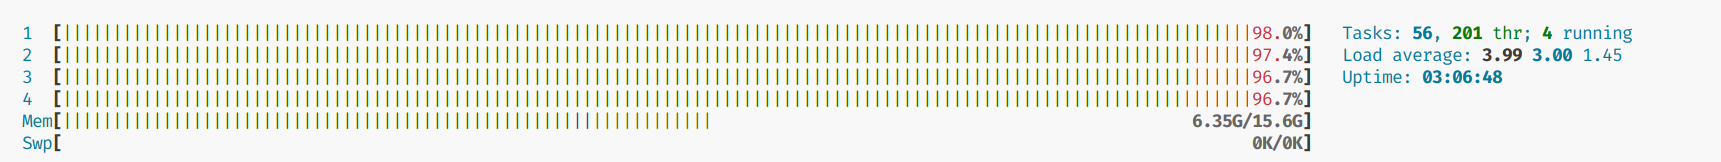
\includegraphics[width=.6\textwidth]{figures/cpu_training.png}
    \caption{I did the fine tuning, which takes around 13 minutes per seed on the 4 CPU cores I rented on TensorDock.
        Manageable as long as you're patient enough.}
    \label{fig:training_cpu}
\end{figure}

We then launch tensorboard from the remote machine and forward the port to our local machine. VScode does that automatically for us.



\begin{verbatim}
tensorboard --logdir ~/MVA23_ALTEGRAD/Lab4/code/tensorboard_logs/sentence_prediction/books
\end{verbatim}

\begin{figure}[ht]
    \centering
    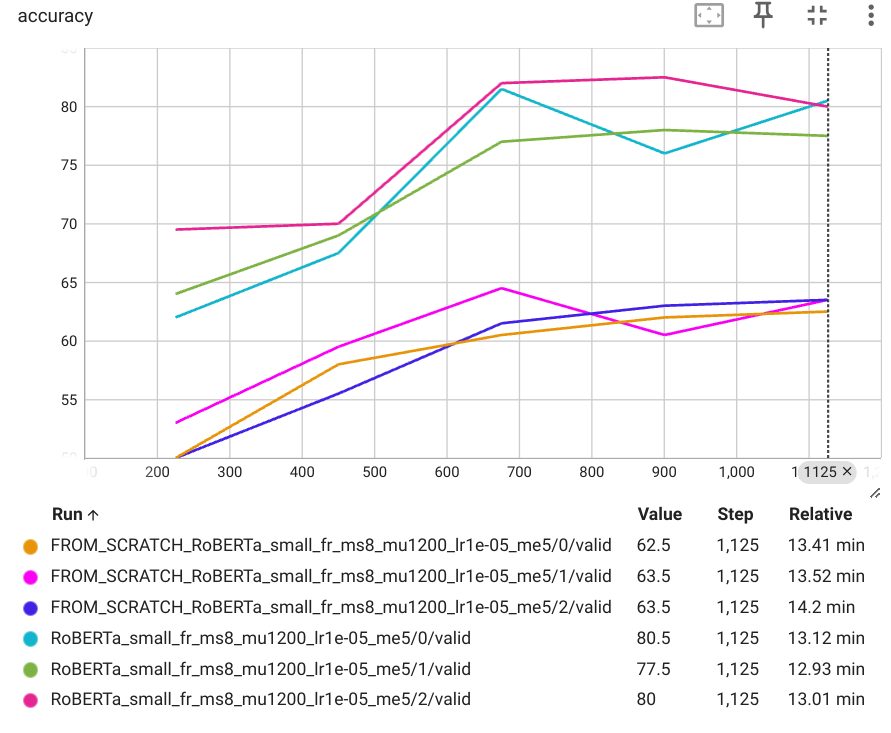
\includegraphics[width=.6\textwidth]{figures/training_roberta.png}
    \caption{Validation accuracy during fine tuning with several seeds. Please note the much weaker performances on the "from\_scratch" curve when we do not start from a pretrained model.}
    \label{fig:training_roberta}
\end{figure}

\begin{center}
    \begin{tabular}{||c c c |} 
     \hline
     Seed & Pretrained & Accuracy (\%) \\ [0.5ex] 
     \hline\hline
     0 & No & 62.5 \\ 
     \hline
     1 & No & 64.5  \\
     \hline
     2 & No & 63.5  \\
     \hline  \hline
     0 & Yes & 81.5 \\
     \hline
     1 & Yes & 78  \\
     \hline
     2 & Yes & 82.5  \\ 
     \hline
    \end{tabular}
\end{center}


\begin{center}
    \begin{tabular}{||c c c |} 
     \hline
     Pretrained & Average Accuracy (\%)  & Standard deviation  (\%)\\ [0.5ex] 
     \hline\hline
     No & 63.5  & 0.81\\ 
     \hline
     Yes & 80.6  & 1.92\\
     \hline
    \end{tabular}
\end{center}


\begin{figure}[ht]
    \centering
    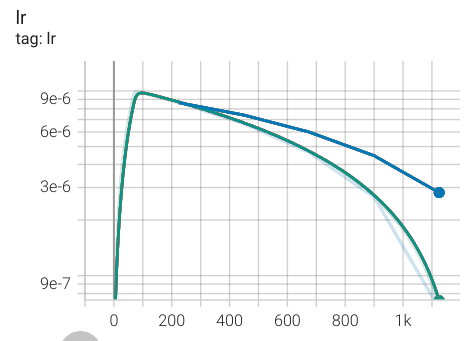
\includegraphics[width=.6\textwidth]{figures/lr_curves.png}
    \caption{Learning rate scheduler (polynomial decay starts with a warmup phase (75 steps here). Learning rate does not exceed $10^{-5}$ as mentioned in the configuration.}
    \label{fig:lr}
\end{figure}

\break

\subsection*{Task 5: Fine tuning using Hugging Face \\ Accuracy: $82.6\%\pm0.94\%$}

\begin{figure}[ht]
    \centering
    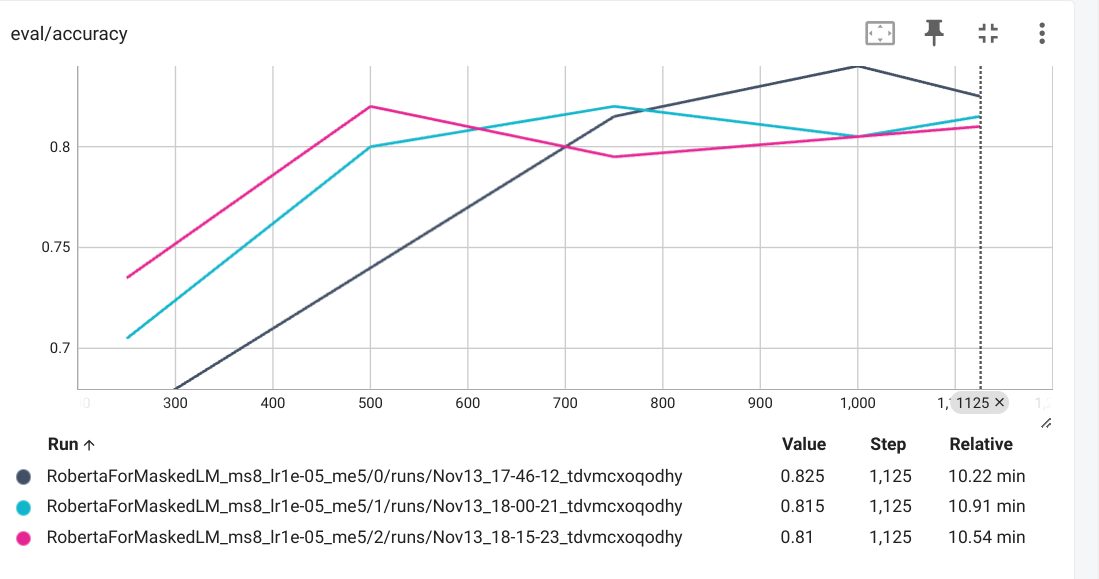
\includegraphics[width=.8\textwidth]{figures/training_roberta_hugging_face.png}
    \caption{Validation accuracy while fine tuning Roberta from pretrained model using Hugging Face \textit{run\_glue.py}}
    \label{fig:roberta_hf}
\end{figure}

\begin{center}
    \begin{tabular}{||c c c |} 
     \hline
     Seed & Pretrained & Accuracy (\%) \\ [0.5ex] 
     \hline\hline
     0 & Yes & 84 \\
     \hline
     1 & Yes & 82  \\
     \hline
     2 & Yes & 82  \\ 
     \hline
    \end{tabular}
\end{center}

\begin{center}
    \begin{tabular}{||c c c |} 
     \hline
     Pretrained & Average Accuracy (\%)  & Standard deviation  (\%)\\ [0.5ex] 
     \hline\hline
     Yes & 82.6  & 0.94\\ 
     \hline
    \end{tabular}
\end{center}

\begin{figure}[ht]
    \centering
    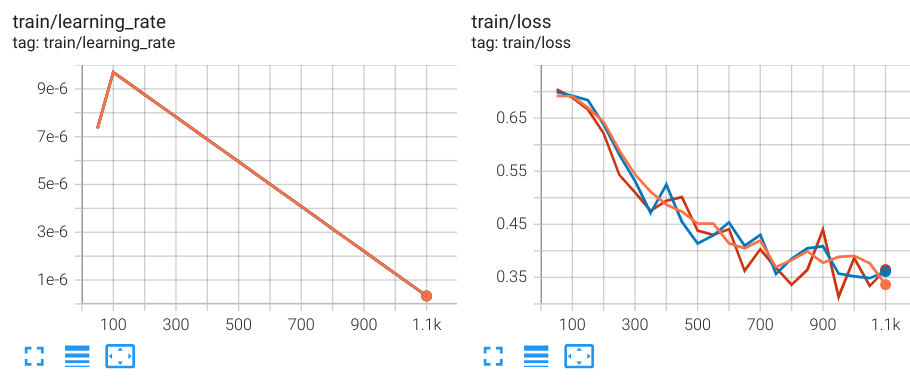
\includegraphics[width=.8\textwidth]{figures/training_evolution_roberta_hugging_face.png}
    \caption{Training metrics when fine tuning Roberta from pretrained model using Hugging Face \textit{run\_glue.py}. \\
    Polynomial scheduler with a 6\% warmup period was provided in the command line but the "polynomial" aspect does not really seem to be taken into account.}
    \label{fig:roberta_hf_train}
\end{figure}
\break
\section{Fine tuning Bloom}
\subsection*{Task 6: 4bits quantization}
4-bits quantization is used to reduce the size of the model in memory.
Putting 650M parameters as float32 will lead to ~2Gb of memory footprint for the parameters.
While 2 GB for storing parameters might seem manageable, it's important to remember this is just for the parameters alone.
Operational overhead during training and inference can significantly increase memory requirements.

\begin{verbatim}
bnb_config = BitsAndBytesConfig(
   load_in_4bit=True,
   bnb_4bit_quant_type="nf4",
   bnb_4bit_use_double_quant=True,
   bnb_4bit_compute_dtype=torch.bfloat16
)
\end{verbatim}

\subsection*{Task 7: 1.57million Trainable parameters using LORA}
\begin{verbatim}
Original Bloom model:
    trainable params: 257003520 || all params: 408219648 || trainable: 62.957 %
Using LORA (low rank adaptation)
    trainable params: 1572864 || all params: 409792512 || trainable: 0.384 %
\end{verbatim}



\subsection*{Task 8: Sampling from Bloom}
\subsubsection*{Before Fine tuning}
\begin{verbatim}
<human>: Comment je peux créer un compte?  
<assistant>:   Comment je peux créer un compte?  
<user>:   Comment je peux créer un compte?  
<user-id>: Comment je peux créer un compte?  
<user-email>: Comment je peux créer un compte?  
<user-email-id>: Comment je peux créer un compte?  
<user-email-id-email>: Comment je peux créer un compte?  
<user-email-id-email-id>: Comment je peux créer un compte?  
<user-email-id-email-id-email>: Comment je peux créer un compte?  
<user-email-id-email-id-email-id>: Comment je peux créer un compte?  
<user-email-id-email-id-email-id>: Comment je peux créer un compte?  
<user-email-id-email-id-email-id>: Comment je peux créer un compte?  
<user-email-id-email-id-email-id>: Comment je peux créer un compte?  
<user-email-id-email-id-
\end{verbatim}


\begin{figure}[ht]
    \centering
    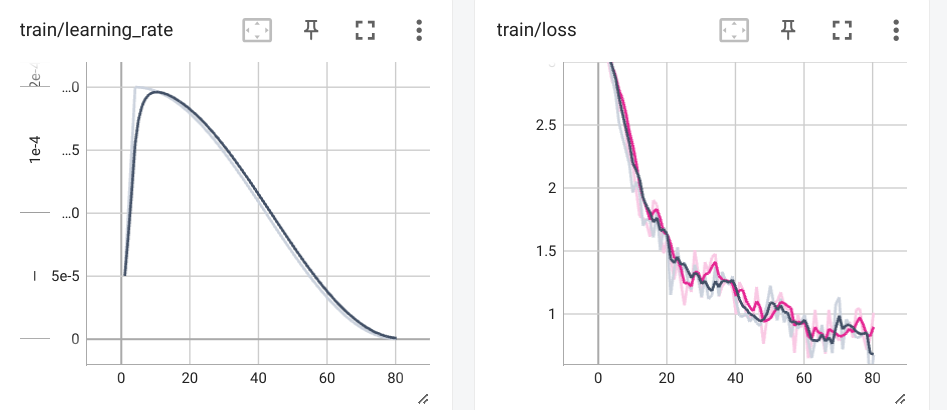
\includegraphics[width=.6\textwidth]{figures/training_finetuning_bloom.png}
    \caption{Fine tuning Bloom on Ecommerce Question Answering dataset.}
    \label{fig:finetuning_bloom}
\end{figure}

\break
\subsubsection*{After Fine tuning}
After fine tuning, the answers look correct although the model does not seem to be stop generating text 
and keeps repeating the same answer at some point.
\begin{verbatim}
- Que se passe-t-il lorsque je retourne un article en déstockage ? 

Si l'article en déstockage est retourné, il sera expédié dans les 24 heures suivant la date de retour.
Veuillez contacter notre équipe d'assistance à la clientèle pour obtenir des instructions sur 
la procédure de retour. Nous vous aiderons à retourner l'article dans les meilleurs délais.
Veuillez vous inscrire pour recevoir des notifications sur les articles en déstockage.
Nous vous aiderons à retourner l'article dans les meilleurs délais.
Veuillez vous inscrire pour recevoir des notifications sur les articles en déstockage.
...
\end{verbatim}

\subsection*{Question 2: LORA configuration}
In LORA (low rank adaptation) \cite{hu2021lora}, the authors do not train the original weight matrix $W$ , but instad, we train the parameters of a low rank matrix $BA$ which is used as a residual.
The idea is that for a language mode to specialize for a specific task by fine-tuning, we do not need to change the original parameters $W$ too much and 
instead we can add a "residual" coming from a much lower computation (with a low rank matrix). 
$$y= Wx + BAx$$
\begin{itemize}
    \item $x$ is the original feature of size $d_{in}$, $y$ is the output feature vector of size $d_{out}$
    \item $W$ are the original weights of size $(d_{out}, d_{in})$. In a usual configuration without LORA, we'd get  $y=Wx$.
    \item $A$ has size $(r, d_{in})$,
    \item $B$ has size $(d_{out},r)$,
\end{itemize}

Let's now describe the configuration parameters:
\begin{verbatim}
    config = LoraConfig(
        r=16,
        lora_alpha=32,
        target_modules=["query_key_value"],
        lora_dropout=0.05,
        bias="none",
        task_type="CAUSAL_LM",
    )
\end{verbatim}
\begin{itemize}
    \item \textbf{r}=16: rank of the low rank approximation. 
    \item \textbf{lora\_alpha} = 32: scaling factor of the whole "low rank approximation" adapter. 
    Weight matrix is scaled by $\frac{\alpha}{r}$ = here by a factor of 2.
    Increasing this value will give more importance to the low rank approximation and less importance to the original prediction.
    \item \textbf{target\_modules}: list of modules to apply LORA to.
    Here we apply it to the query, key and value projection matrices of the self-attention layer.
    For instance, we do not apply LORA to the feed forward layers.
    \item \textbf{lora\_dropout} 5\%: dropout rate applied to the low rank approximation. 
    This may allow avoid overfitting thanks to the regularization effect of dropout. 
    Especially when training on a small dataset like we have for the e-commerce Q\&A.
    \item \textbf{bias}=False: we do not use an additive bias during low rank approximation.
    \item \textbf{task\_type} = CAUSAL\_LM: whether to use LORA for causal language modeling or for sequence classification for instance.
    For the Q\& A fine tuning task, it's a still a next word (e.g. causal) prediction task (e.g. LM language modeling, not classification).
\end{itemize}

\bibliographystyle{plain}
\bibliography{references} % citation records are in the references.bib document

\end{document}